
\section{Simulation results and Analysis} 
\label{Sec:exp}
The forestry crane simulator is built using Mujoco 3.0 \cite{todorov2012mujoco} in an AMD Threadripper 7980X with 64GB memory of RAM and the GeForce RTX 4090. We use the Conjugate gradient (CG) solver \cite{nazareth2009conjugate} with the implicit Euler integration method with a sampling time of $\SI{5}{\milli\second}$ for solving the multi-contact system dynamics. Since the maximum simulation time for an episode is $\SI{15}{\second}$, the maximum episode length is $H = 15/0.005 = 3000$ steps. 
Using the standard PPO algorithm in the open-source package Stable-baseline3 \cite{raffin2021stable}, the mPPO is implemented by considering the Beta distribution and (\ref{eq: robust ppo}). We utilize $42$ parallel environments in the training process of $5\cdot 10^8$ simulation steps for all tested algorithms. The network architecture, see Figure \ref{fig: overview learning}, has $4$ layers with 256 neurons in each layer. The update interval is $1000$ steps for each rollout.  Additionally, ADAM optimizer is utilized \cite{kingma2014adam} with the learning rate $\lambda = 3\cdot 10^{-4}$ and $30$ mini epochs in each optimization batch. Note that the optimizer will take approximately ${5\cdot 10^8}/(42\times1000) \approx 12000$ update steps by the optimizer. 
\begin{figure}
	\centering
 \scalebox{0.94}{
	\includegraphics[width=0.5\textwidth]{figures/learning-reward-new.png}
 }
	\caption{Evolution of cumulative rewards over $12000$ update steps of the optimizer.}
    \label{fig: episode reward}
\end{figure}
\subsection{Benchmarking results}
The cumulative rewards over the whole training process are depicted in Figure \ref{fig: episode reward}, with four different algorithms, i.e., Trust Region Policy Optimization (TRPO) \cite{schulman2015trust}, Recurrent PPO \cite{huang202237}, PPO \cite{schulman2017proximal}, and the proposed mPPO. In the beginning, early terminations, see Subsection \ref{sec: early termination}, are often triggered. This leads to short episode lengths at the beginning of the training process. We achieve better results with the PPO and the mPPO algorithm than the TRPO and the RecurrentPPO algorithms. 
This could be because the agent is not encouraged to explore the large action space by these two latter algorithms. Although we achieve better results with the mPPO than the conventional PPO, the agent sometimes heuristically explores too much, which can lead to a sudden decrease in the average episode length and the cumulative reward. 
\iffalse
    \begin{figure}
    	\centering
    	\includegraphics[width=0.5\textwidth]{figures/episode_length.png}
            %\def\svgwidth{1\columnwidth}
            %\input{doc/tex/graphics/KinematicChain.pdf_tex}
    	\caption{Evolution of episode lengths over $12500$ update steps of the optimizer.}
        \label{fig: episode length}
    \end{figure}
\fi


It is worth noting that the multi-contact system dynamics are processed in the CPU, while the RL algorithms are executed in the GPU. The computing speeds (including CPU and GPU time) when utilizing mPPO and the PPO algorithms are nearly similar, with $6500$ steps per second. On the other hand, the computing speeds of TRPO and RecurrentPPO are much slower, with $2500$ and $1500$ steps per second. For $5\cdot10^8$ steps, the mPPO and PPO spend approximately $21.5$ hours of training, whereas the TRPO and RecurrentPPO need approximately $56$ and $92.3$ hours, respectively. 


\subsection{Insights into the learned grasping skill}
In Figure \ref{fig: grasping skill 1}, an example of a demonstration is performed by the trained agent with mPPO for grasping a wood log with a diameter $d=\SI{0.4}{\meter}$. The forestry crane quickly approaches the log and aligns the grapple with the log's orientation, see Figure \ref{fig: grasping skill 1}(a)-(c). 
It is worth noting that the agent does not use a conventional grasping technique, such as perfectly aligning the grapple with the tree log. Instead, the agent approaches the tree log in a versatile way while moving as long as the vector $\mathbf{e}_{C,x}$ is parallel to the unit length vector of the tree log $\mathbf{e}_{l,y}$, as defined by (\ref{eq: angle distance}). Whenever the combined distance $d_\mathrm{combine}$ from (\ref{eq: d combine}) is below a certain threshold, i.e., $r_\mathrm{distance} \rightarrow 1$, see (\ref{eq: r_distance}), the grapple starts closing, followed by a lifting action; see Figure \ref{fig: grasping skill 1}(d)-(f). 
%Interestingly, the agent slightly leans on the left side to roll the wood log, see Figure \ref{fig: grasping skill 1}(d), then quickly closes the grapple to grasp the log fully, Figure \ref{fig: grasping skill 1}(d). 
\iffalse
    Note that not all demonstrations have shown the same behavior. For instance, to grasp a log with the diameter $d=\SI{0.3}{\meter}$ while approaching and aligning to the wood log pose, the agent slightly lifts the grapple, see Figure \ref{fig: grasping skill 2}(c), to perfectly grasp the wood log without rolling it, see Figure \ref{fig: grasping skill 2}(d). These behaviors are obtained thanks to the agent's ability to explore using the modified PPO algorithm during the training process. 
\fi    
\begin{figure}
\centering
\def\svgwidth{0.8\columnwidth}
\input{figures/overlay_grasping_1_ver2.pdf_tex}
\vspace{0.2cm}
\caption{Sequence of images from a grasping demonstration with the log diameter $d = \SI{0.4}{\meter}$. }
\label{fig: grasping skill 1}
\end{figure}
\iffalse
    \begin{figure*}
    \centering
    \subfigure{
    \def\svgwidth{1.75\columnwidth}
    \input{figures/overlay_grasping_2.pdf_tex}
    }
    \caption{Sequence of images from a grasping demonstration with the log diameter $d = \SI{0.3}{\meter}$. }
    \label{fig: grasping skill 2}
    \end{figure*}
\fi
\definecolor{transfertoclient}{HTML}{ABDDA4}
\definecolor{rendering}{HTML}{2B83BA}
\iffalse
\begin{figure}
    \centering   
    \scalebox{0.8}{
    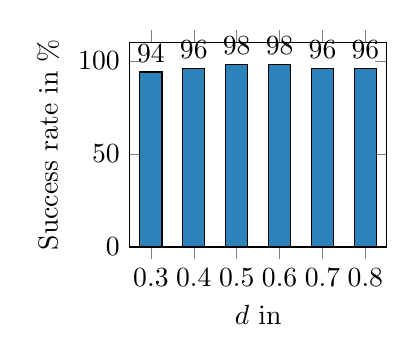
\begin{tikzpicture}
        \begin{axis} [ybar=8pt,
            width=0.4\textwidth,
            bar width = 8pt,
            xtick   =   data,
            nodes near coords,
            ylabel= Success rate in \%,
            xlabel= $d$ in \SI{}{\meter},
            ymin = 0,
            ymax = 110
        ]
            \addplot[fill=rendering] coordinates {  
            (0.3, 94)    %                      
            (0.4, 96)    % 
            (0.5, 98)   % 
            (0.6, 98) 
            (0.7, 96)
            (0.8, 96)};
        \end{axis}
    \end{tikzpicture}
    }
    \caption{Statistical results for grasping logs with different diameter $d$.}
    \label{fig:stats log size}
\end{figure}
\fi

\begin{table}
\caption{Statistical results for grasping logs with different diameter $d$.} 
\vspace{1ex}
\centering
\renewcommand
\tabcolsep{4.5pt}
\hspace{1ex}
% \resizebox{\linewidth}{!}{
\begin{tabular}{@{}rcccccc@{}}
\toprule
$d$ in \SI{}{\meter} & 0.3 & 0.4 & 0.5 & 0.6 & 0.7 & 0.8 \cr 
\midrule
success rate (\%)  & 94 & 96 & 98 & 98 & 96 & 96 \\
\bottomrule
\end{tabular}
% }
\label{table:stats log size}
\end{table}
%\subsection{Comparisons}
\subsection{Statistical results}
\label{sec: stats MC}
%To further challenge the agent, we run the Monte Carlo simulation with six different batches with log dimensions range in $d \in \{0.3,...,0.8\}$. 
To challenge the agent, we run a Monte Carlo simulation with six batches with log diameters in the range $d \in \{0.3,...,0.8\} \SI{}{\meter}$. We collect $100$ trials in each batch by randomizing the initial configuration for the forestry crane and the log's pose. 
A trial is considered a success if the agent can reach the log within the time limit of \SI{6}{\second} and fully grasp the log in $\SI{9}{\second}$. Even if the agent can completely capture the tree log within the time limit, if it misses the center of the wood log by a particular threshold value, we also consider this a failed trial. In Table \ref{table:stats log size}, the statistical results of the mentioned Monte Carlo simulation are shown. For the smallest log diameter $d = \SI{0.3}{\meter}$, there are $6$ failed trials in which slowly closing the grapple behavior leads to exceeding the time limit of $\SI{9}{\second}$. With larger logs, failures only occur if the agent misses the center of the log, followed by the excessive swinging motion of the unactuated joints during lifting. Overall, the trained agent achieves a success rate of over $96\%$  for this Monte Carlo simulation. 

\iffalse
    We validate our method with different observation modalities and train new models with the same $5.10^8$ steps. In Figure \ref{fig: camera placement}, two RGD-D cameras are placed under the gripper and at the control box. The camera images are passed through a standard CNN feature extractor network and concatenated with other observations. Initially, we assume the observation space contains the images (RGB and depth) of two cameras and the crane state. In this case, the reward function only includes the lifting condition since we do not know the position of the trunk. The success rate of 600 trials (100 trials for each trunk diameter) is about $52.5\%$, see Table \ref{table:stats observation type}. With this type of observation, the agent is not able to explore the large state space of the crane because it lacks important information, such as the relative distance to the target. Next, we integrate the RGB-D data from the two cameras and the observation mentioned in subsection \ref{sec: observation}. The success rate is about $95.8\%$, which is quite similar to the result from Table \ref{table:stats log size}. This allows us to confirm that the relative information with respect to the target log, i.e., (\ref{eq: angle distance}) and (\ref{eq: d combine}), plays a key role in the agent's learning process. A video with several demonstrations can be seen at \href{https://www.acin.tuwien.ac.at/en/d18a/}{https://www.acin.tuwien.ac.at/en/d18a/}. 
    
    
    \begin{table}
    \caption{Statistical results with different observation types.} 
    \vspace{1ex}
    \centering
    \renewcommand
    \tabcolsep{4.5pt}
    \hspace{1ex}
    % \resizebox{\linewidth}{!}{
    \begin{tabular}{@{}rcc@{}}
    \toprule
    obs. case & reward case &  success rate(\%) \cr 
    \midrule
    ours & default & 96.3\\
    cameras + crane states & only lifting & 52.5 \\ % 315 cases - 4070 RTX machine
    ours + cameras & default & 95.8\\ % 575 cases - 4070 RTX machine
    \bottomrule
    \end{tabular}
    % }
    \label{table:stats observation type}
    \end{table}
    
    
    \begin{figure}
    \centering
    \def\svgwidth{0.6\columnwidth}
    \input{figures/camera-observation.pdf_tex}
    \vspace{0.2cm}
    \caption{Example of new observations from two cameras.}
    \label{fig: camera placement}
    \end{figure}
\fi    
\subsection{Bridging Sim-to-real aspect} 
The augmented relative Cartesian distance (\ref{eq: relative distance}) and the angular distance function (\ref{eq: angle distance}) are important as they lead the agent directly to the goal, especially in model-free RL. 
The same assumption is commonly employed in indoor robot manipulation tasks \cite{mu2021maniskill} or large-scale robot manipulation \cite{andersson2021reinforcement}. Learning with solely visual input only works in generative AI scenarios where the agent can learn from expert demonstration while observing multimodal data, e.g., RGB-D and force/torque profiles. 

However, we recognized that assuming a known log's pose, which leads to (\ref{eq: relative distance}) and (\ref{eq: angle distance}), significantly contributes to the sim-to-read gap. %Therefore, we further stress our agent by adding error measurements to (\ref{eq: relative distance}) and (\ref{eq: angle distance}). Specifically, maximum 10\% errors are added in the following 
In order to account for this effect, we add measurement errors to (\ref{eq: relative distance}) and (\ref{eq: angle distance}) in the form
\begin{subequations}
\begin{align}
    \bm{\Delta}_p &\leftarrow  \bm{\Delta}_p + \epsilon_p\bm{\Delta}_p s(\bm{\Delta}_p)\:, \\
    \Delta_\psi &\leftarrow  \Delta_\psi + \epsilon_o\Delta_o s(\bm{\Delta}_p) \:,
\end{align}
\end{subequations}
where $\epsilon_p$ and $\epsilon_o$ are random values drawn from a uniform distribution $U(-0.1,0.1)$. Note that $s(\bm{\Delta}_p)$ is the quadratic decay function, expressed as $s(\bm{\Delta}_p) = (||\bm{\Delta}_p||/{d_{max}})^2$, with $d_{max}=\SI{8}{\meter}$ in our setup. 
%at greater distances, which scales down to zero as the distance to the target decreases 
This is a practical assumption since, in our real setup, two RGB-D cameras, attached to the control box and the gripper, are employed for log pose detection, see Figure \ref{fig: example mujoco}(b). The same Monte Carlo simulation as in Subsection \ref{sec: stats MC} is performed with six batches (100 trials in each batch) of log diameters $d \in\{0.3,...,0.8\}$. The statistical results of this test are shown in Table \ref{tab:table-new}. Most of the failed cases with small logs, $d= 0.3$ and $d=0.4$, are due to exceeding the time limit of $\SI{9}{\second}$. On the other hand, with larger diameter logs $d \geq 0.5$, failed cases are caused by a miss-aligned grasp due to an orientation error. Overall, the agent achieves a success rate of $\approx 92\%$ for all cases. %A video with several demonstrations can be seen at \href{https://www.acin.tuwien.ac.at/en/d18a/}{https://www.acin.tuwien.ac.at/en/d18a/}. 
\begin{table}
\caption{Statistical results of adding errors to the pose measurement.} 
\vspace{1ex}
\centering
\renewcommand
\tabcolsep{4.5pt}
\hspace{1ex}
% \resizebox{\linewidth}{!}{
\begin{tabular}{@{}rcccccc@{}}
\toprule
$d$ in \SI{}{\meter} & 0.3 & 0.4 & 0.5 & 0.6 & 0.7 & 0.8 \cr 
\midrule
success rate (\%)  & 88 & 94 & 93 & 93 & 92 & 91 \\
\bottomrule
\label{tab:table-new}
\end{tabular}
\end{table}

